\documentclass[12pt]{report}

% --- Paquetes esenciales ---
\usepackage[spanish]{babel}
\usepackage[utf8]{inputenc}
\usepackage{amsmath,amssymb,amsthm}
\usepackage{graphics,graphicx,subfigure}
\usepackage{lipsum,array,multicol,enumerate,enumitem}
\usepackage[framemethod=TikZ]{mdframed}
\usepackage[a4paper, margin=1.5cm]{geometry}
\usepackage{tikz,pgffor,ifthen}
\usepackage{hyperref,longtable,listings}
\usepackage{booktabs}
\usepackage{eso-pic}
\usepackage{bbm}

% --- Gestión marca de agua --- 
\AddToHook{shipout/foreground}{%
    \begin{tikzpicture}[remember picture,overlay]
        \node at (current page.center){
            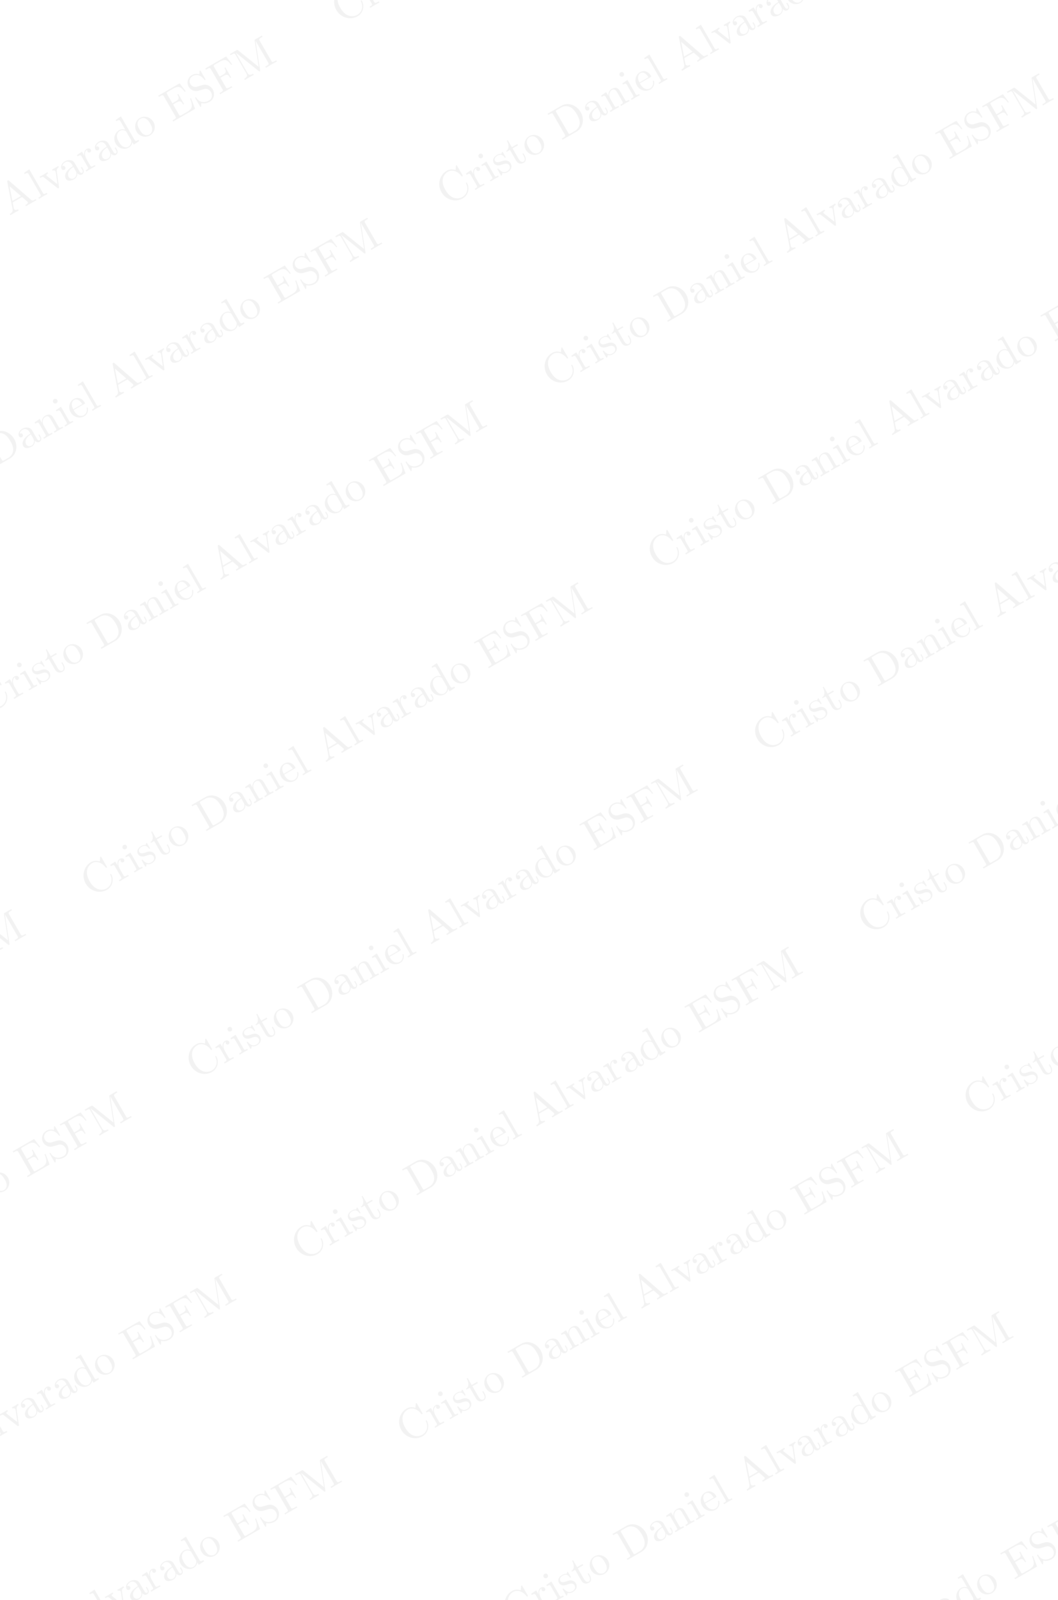
\includegraphics[width=\paperwidth,height=\paperheight,keepaspectratio]{watermark-1.png}
        };
    \end{tikzpicture}%
}

% --- Configuración de hipervínculos ---
\hypersetup{
    colorlinks=true,
    linkcolor=black,
    filecolor=magenta,      
    urlcolor=cyan
}

% --- Estilo para listings (código) ---
\definecolor{listing-background}{HTML}{F7F7F7}
\definecolor{listing-rule}{HTML}{B3B2B3}
\definecolor{listing-numbers}{HTML}{B3B2B3}
\definecolor{listing-text-color}{HTML}{000000}
\definecolor{listing-keyword}{HTML}{435489}
\definecolor{listing-keyword-2}{HTML}{1284CA}
\definecolor{listing-keyword-3}{HTML}{9137CB}
\definecolor{listing-identifier}{HTML}{435489}
\definecolor{listing-string}{HTML}{00999A}
\definecolor{listing-comment}{HTML}{8E8E8E}

\lstdefinestyle{myStyle}{
    language         = C++,
    alsolanguage     = scala,
    numbers          = left,
    xleftmargin      = 2.7em,
    framexleftmargin = 2.5em,
    backgroundcolor  = \color{gray!15},
    basicstyle       = \color{listing-text-color}\linespread{1.0}\ttfamily,
    breaklines       = true,
    frameshape       = {RYR}{Y}{Y}{RYR},
    rulecolor        = \color{black},
    tabsize          = 2,
    numberstyle      = \color{listing-numbers}\linespread{1.0}\small\ttfamily,
    aboveskip        = 1.0em,
    belowskip        = 0.1em,
    abovecaptionskip = 0em,
    belowcaptionskip = 1.0em,
    keywordstyle     = {\color{listing-keyword}\bfseries},
    keywordstyle     = {[2]\color{listing-keyword-2}\bfseries},
    keywordstyle     = {[3]\color{listing-keyword-3}\bfseries\itshape},
    sensitive        = true,
    identifierstyle  = \color{listing-identifier},
    commentstyle     = \color{listing-comment},
    stringstyle      = \color{listing-string},
    showstringspaces = false,
    label            = lst:bar,
    captionpos       = b,
}
\lstset{style = myStyle}

% --- Redefiniciones de encabezados de capítulo y sección ---
\makeatletter
\def\@makechapterhead#1{%
  {\parindent \z@ \raggedright
    \reset@font
    \hrule
    \vspace*{10\p@}%
    \par
    \center \LARGE \scshape \@chapapp{} \huge \thechapter
    \vspace*{10\p@}%
    \par\nobreak
    \vspace*{10\p@}%
    \par
    \vspace*{1\p@}%
    \hrule
    \vspace*{60\p@}
    \Huge #1\par\nobreak
    \vskip 50\p@
  }}
\makeatother

% --- Entornos personalizados ---
\newtheoremstyle{largebreak}{}{ }{\normalfont}{}{\bfseries}{}{\newline}{}
\theoremstyle{largebreak}

\newmdtheoremenv[hidealllines=true,roundcorner=5pt,backgroundcolor=gray!60!red!30]{exa}{Ejemplo}[section]
\newmdtheoremenv[hidealllines=true,roundcorner=5pt,backgroundcolor=gray!50!blue!30]{obs}{Observaci\'on}[section]
\newmdtheoremenv[hidealllines=true,roundcorner=5pt,backgroundcolor=green!50!blue!30]{preg}{Pregunta}[section]
\newmdtheoremenv[hidealllines=true,roundcorner=5pt,backgroundcolor=yellow!40]{idea}{Idea}[section]
\newmdtheoremenv[rightline=false,leftline=false]{theor}{Teorema}[section]
\newmdtheoremenv[rightline=false,leftline=false]{propo}{Proposici\'on}[section]
\newmdtheoremenv[rightline=false,leftline=false]{cor}{Corolario}[section]
\newmdtheoremenv[rightline=false,leftline=false]{lema}{Lema}[section]
\newmdtheoremenv[roundcorner=5pt,backgroundcolor=gray!30,hidealllines=true]{mydef}{Definici\'on}[section]
\newmdtheoremenv[roundcorner=5pt]{excer}{Ejercicio}[section]

% --- Comandos auxiliares ---
\def\proof{\paragraph{Demostraci\'on:\\}}
\def\endproof{\hfill$\blacksquare$}
\def\sol{\paragraph{Soluci\'on:\\}}
\def\endsol{\hfill$\square$}

\newcommand\abs[1]{\ensuremath{\left|#1\right|}}
\newcommand\norm[1]{\ensuremath{\|#1\|}}
\newcommand\divides{\ensuremath{\bigm|}}
\newcommand\cf[3]{\ensuremath{#1:#2\rightarrow#3}}
\newcommand\contradiction{\ensuremath{\#_c}}
\newcommand\natint[1]{\ensuremath{\left[\big|#1\big|\right]}}
\newcommand{\bbm}[1]{\ensuremath{\mathbbm{#1}}}

\newcounter{figcount}
\setcounter{figcount}{1}

\renewcommand{\lstlistingname}{Código}
\renewcommand{\lstlistlistingname}{Lista de \lstlistingname s}

% --- Comienzo del documento ---
\begin{document}

\setlength{\parskip}{5pt}
\setlength{\parindent}{12pt}
\title{T\'itulo o Nombre de las notas}
\author{Cristo Daniel Alvarado}
\maketitle

\tableofcontents

\lstlistoflistings

\newpage

\chapter{Conjuntos Convexos}

\section{Propiedades Básicas}

\begin{mydef}[\textbf{Conjunto Convexo}]
    Sea $C\subseteq\bbm{R}^n$ un conjunto no vacío. Decimos que $C$ es un conjunto convexo si $[a,b]\subseteq C$, donde:
    \begin{equation*}
        [a,b]=\left\{ta+(1-t)b\Big|t\in[0,1] \right\}
    \end{equation*}
\end{mydef}

\begin{exa}
    El conjunto $\bbm{R}^n$ es convexo. También lo son $[a,b]\subseteq\mathbb{R}^n$ y $\left\{a\right\}$, para todo $a,b\in\bbm{R}^n$.
\end{exa}

Los conjuntos convexos resultan relevantes pues justamente en vecindades convexas podemos definir conceptos como derivadas direccionales, gradientes, etc\dots

Una propiedad que podemos definir en un conjunto convexo es el siguiente:

\begin{mydef}[\textbf{Punto Extremo}]
    Sea $C\subseteq\bbm{R}^n$ un conjunto convexo. Decimos que un punto $x\in C$ es \textbf{punto extremo de $C$} si no existen $y,z\in C$ tales que $x\in(y,z)$, donde:
    \begin{equation*}
        (y,z)=\left\{ty+(1-t)z\Big|t\in(0,1) \right\}
    \end{equation*}
\end{mydef}

\begin{exa}
    El conjunto $(-\infty,a]\subseteq\bbm{R}^n$ dado por:
    \begin{equation*}
        (-\infty,a]=\left\{ta\in\bbm{R}^n\Big|t\leq1 \right\}
    \end{equation*}
    es convexo y tiene como único punto extremo a $a$. También, $[a,b]$ tiene como puntos extremos a $a$ y $b$.

    En cambio, el conjunto $(a,b)$ es convexo pero no tiene puntos extremos.
\end{exa}

\begin{lema}
    Sea $C\subseteq\bbm{R}^n$ subconjunto convexo y sea $x\in C$ tal que $x$ no es extremo. Entonces, existen $y,z\in C$ tales que:
    \begin{equation*}
        x=\frac{y+z}{2}
    \end{equation*}
\end{lema}

\begin{proof}
    Como $x\in C$ no es extremo, existen $y_0,z_0\in C$ y $t\in(0,1)$ tales que:
    \begin{equation*}
        x=ty_0+(1-t)z_0
    \end{equation*}
    Si $t=\frac{1}{2}$ hemos terminado. En caso contrario, sea $s=\max\left\{t,1-t\right\}$. Se tienen dos casos:
    \begin{itemize}
        \item $s=t$, tomemos $y=y_0$ y $z=\frac{1-t}{t}z_0+\left(1-\frac{1-t}{t}\right)x$ (se verifica rápidamente que ambos están en $C$, pues están en $[y_0,z_0]$), entonces:
        \begin{equation*}
            \begin{split}
                \frac{y+z}{2}&=\frac{y_0+\frac{1-t}{t}z_0+\left(1-\frac{1-t}{t}\right)x}{2}\\
                &=\frac{y_0+\frac{1-t}{t}z_0+\left(1-\frac{1-t}{t}\right)(ty_0+(1-t)z_0)}{2}\\
                &=\frac{y_0+\frac{1-t}{t}z_0+\left(t-\frac{1-t}{t}t\right)y_0+\left(1-t-\frac{1-t}{t}(1-t)\right)z_0}{2}\\
                &=\frac{2ty_0+2(1-t)z_0}{2}\\
                &=ty_0+(1-t)z_0\\
                &=x\\
            \end{split}
        \end{equation*}
        \item $s=1-t$, tomemos $z=z_0$ y $y=\frac{t}{1-t}y_0+\left(1-\frac{t}{1-t}\right)x$ (se verifica rápidamente que ambos están en $C$, pues están en $[y_0,z_0]$), haciendo el procedimiento análogo al caso anterior, se llega a que $\frac{y+z}{2}=x$.
    \end{itemize}
    Por ambos incisos se sigue el resultado.
\end{proof}

\begin{theor}[\textbf{Propiedades Básicas de los Puntos Extremos}]
    Si $C\subseteq\bbm{R}^n$ es acotado, convexo y cerrado, entonces $C$ tiene al menos un punto extremo. Más aún, si $C$ tiene más de un punto, entonces debe tener al menos dos puntos extremos.
\end{theor}

\begin{proof}
    Sea $C\subseteq\bbm{R}^n$ un conjunto acotado, cerrado y convexo. Consideremos la función $\cf{f}{C\times C}{\bbm{R}}$ dada por:
    \begin{equation*}
        f(x,y)=\norm{x-y}
    \end{equation*}
    $f$ es una función continua en un conjunto compacto, por lo que alcanza su máximo en algún punto $(x_0,y_0)\in C\times C$. Tenemos dos casos:
    \begin{itemize}
        \item $f(x_0,y_0)=0$: Se sigue que $x_0=y_0$, luego $C$ tiene un punto. Se sigue así que $C$ tiene al menos un punto extremo.
        \item $f(x_0,y_0)>0$: Afirmamos que $x_0$ y $y_0$ son puntos extremos de $C$. Supongamos que alguno de ellos no es un punto extremo, digamos $x_0$, entonces por el lema anterior existen $x_1,x_2\in C$ tales que:
        \begin{equation*}
            x_0=\frac{x_1+x_2}{2}
        \end{equation*}
        Si alguno de estos dos puntos es extremo, hemos terminado, por lo que supongamos que ninguno de estos dos es extremo. Por la identidad del paralelogramo y ya que $f$ alcanza su máximo en $(x_0,y_0)$, se tiene que:
        \begin{equation*}
            \begin{split}
                2\norm{x_0-y_0}^2&\geq\norm{x_1-y_0}^2+\norm{x_2-y_0}^2\\
                &=\frac{1}{2}\norm{x_1+x_2-2y_0}^2+\frac{1}{2}\norm{x_1-x_2}^2\\
                &=2\norm{x_0-y_0}^2+\frac{1}{2}\norm{x_1-x_2}^2\\
            \end{split}
        \end{equation*}
        Por tanto, $\norm{x_1-x_2}^2=0$, lo cual implica que $x_1=x-2$, lo cual es una contradicción. Por tanto, $x_0$ es un punto extremo de $C$. Análogamente, se prueba que $y_0$ es un punto extremo de $C$.
    \end{itemize}
    Por los dos incisos se sigue el resultado.
\end{proof}

Uno de los resultados más fundamentales en la teoría es el siguiente:

\begin{theor}
    Sea $C\subseteq\bbm{R}^n$ un subconjunto convexo, cerrado y acotado. Entonces, si $C$ tiene $m$ puntos extremos, digamos $x_1,\dots,x_m$, cualquier punto $x\in C$ como:
    \begin{equation*}
        x=\sum_{i=1}^{m}\alpha_ix_i,\quad\text{con}\quad\sum_{i=1}^{m}\alpha_i=1,\quad\alpha_i\geq0\quad\forall i=1,\dots,m
    \end{equation*} 
\end{theor}

La prueba requiere elementos de análisis funcional y demás herramientas avanzadas, por lo que no se presenta aquí. Sin embargo, este resultado puede consultarse en la siguiente monografía: \href{https://www.mate.unlp.edu.ar/publicaciones/08112010160003.pdf}{Teorema de Krein-Milman}. En esta monografía se presenta una versión más general del teorema (en espacios topológicos localmente convexos).



\end{document}